% !TeX root = main.tex
%%%%%%%%%%%%%%%%%%%%%%%%% PREAMBLE %%%%%%%%%%%%%%%%%%%%%%%%%%%%%%%%
%%%%%%%%%%%%%%%%%%%%%%%% BASIC DOCUMENT SETUP %%%%%%%%%%%%%%%%%%%%%
\documentclass[a4paper]{report}
\usepackage[utf8]{inputenc}
\usepackage[english]{babel}

%%%%%%%%%%%%%%%%%%%%%%%%%% PACKAGES %%%%%%%%%%%%%%%%%%%%%%%%%%%%%%%
\usepackage{datetime}
\usepackage{datenumber}
\usepackage{parskip}
\usepackage{forest}
\usepackage{svg}        % makes it possible to use svg files
\usepackage{graphics}
\usepackage{multicol}
\usepackage{icomma}
\usepackage{microtype}  % microscopic typography refinement
\usepackage{lastpage}   % used to reference last page in footer
\usepackage{fancyhdr}   % Header
\usepackage{tcolorbox}
\usepackage{quiver}
\usepackage{amssymb}
\usepackage[Bjornstrup]{fncychap}
\usepackage[titles]{tocloft}
\usepackage{amsmath}    % mathematics for matrices and more
\usepackage{amsfonts}
\usepackage{csquotes}
\usepackage{morewrites}

\usepackage{tikz}
\usetikzlibrary{calc}   % position og tikz labels
\usetikzlibrary{arrows.meta}
\usetikzlibrary{decorations.pathreplacing,calligraphy}

\usepackage{float}
\usepackage{pgfplots}
\pgfplotsset{compat=1.17}
\usepackage{xcolor}
\definecolor{blueplot}{RGB}{60, 64, 198}
\definecolor{yellowplot}{RGB}{255, 211, 42}
\definecolor{redplot}{RGB}{255, 63, 52}
\definecolor{greenplot}{RGB}{5, 196, 107}
\definecolor{greyplot}{RGB}{72, 84, 96}

\usepackage{siunitx}
\sisetup{%quotient-mode=fraction,
		output-decimal-marker = {,},
		per-mode = fraction,
		separate-uncertainty = true,
		multi-part-units=single,
		exponent-product = \cdot,
		range-phrase=--}
		
\usepackage{minted} % Syntax highlighting 
%\usemintedstyle{monokai}
\setminted[]{breaklines, 
    breakafter=d,
    frame=lines,
    framesep=2mm,
    baselinestretch=1.2,
    fontsize=\footnotesize,
    tabsize=4,
    linenos}


\makeatletter
\renewcommand\@makefnmark{\textsuperscript{[\@thefnmark]}}
\renewcommand\@makefntext[1]{\textsuperscript{[\@thefnmark]}\enspace #1}
\makeatother

\usepackage[hidelinks, linktoc=all]{hyperref} % links, references, \ref{...}
\hypersetup{
    colorlinks = true,
    linkcolor = blue,
    citecolor = blue,
    urlcolor = blue
}
\urlstyle{same}

\usepackage{todonotes}

\usepackage{subcaption}

\usepackage{forest}

\usepackage{lipsum}  

\usepackage{wrapfig}

\usepackage[export]{adjustbox}


\usepackage[pdf]{graphviz}

%%% Helper code for Overleaf's build system to
%%% automatically update output drawings when
%%% code in a \digraph{...} is modified
\usepackage{xpatch}
\makeatletter
\newcommand*{\addFileDependency}[1]{% argument=file name and extension
  \typeout{(#1)}
  \@addtofilelist{#1}
  \IfFileExists{#1}{}{\typeout{No file #1.}}
}
\makeatother
\xpretocmd{\digraph}{\addFileDependency{#2.dot}}{}{}

\usepackage[block=ragged, sorting=nyt, style=authoryear-ibid, backend=biber]{biblatex}
\setlength\bibitemsep{1.5\itemsep}
\addbibresource{mybib.bib}

%%%%%%%%%%%%% ACTUAL VISIBLE CONTENT %%%%%%%%%%%%%%%%%%%%%%%%%%%%%%
\begin{document}
\begin{titlepage}
    \begin{centering}
    \vspace*{-20px}\large Department of Mathematics \& Computer Science\\
    University of Southern Denmark $|$ IMADA \\
    \today \\
    
    \vspace{\fill}
    
    \huge{\bf  Capture the Flag Platform} \\
    \Large{\bf SPDM801: Master's Thesis}
    
    \vspace{\fill}
    
    \begin{minipage}{0.45\textwidth} 
    \begin{flushleft}
        \Large
        \textit{Author}\\
        KIAN BANKE LARSEN\\
        kilar20@student.sdu.dk
    \end{flushleft}
    \end{minipage}
    
    \vspace{\fill}
    
    \begin{minipage}{0.45\textwidth}
    \begin{flushleft}
        \Large
        \textit{Supervisor}\\
        Jacopo Mauro\\
        Professor
    \end{flushleft}
    \end{minipage}
    
    \vspace{\fill}
    
    \includesvg[width=.4\textwidth]{template/SDU.svg}
    
    \vspace*{0.1cm}
    
    \end{centering}
    
    \thispagestyle{empty}
\end{titlepage}

\begin{abstract}
\paragraph{English}

\paragraph{Danish}
\end{abstract}

\chapter*{Acknowledgements}
\thispagestyle{empty}
\clearpage

\pagenumbering{roman}

{ \hypersetup{hidelinks} \tableofcontents \addtocontents{toc}{\vskip-40pt}}

\newpage
\pagenumbering{arabic}
\setcounter{page}{1}

\chapter{Introduction}
Digitalization has become an integral part of our lives. As technology continues to evolve, so do the challenges associated with it. One of the most pressing issues in today's digital landscape is cybersecurity, as it is part of \textit{Europe's digital targets for 2030} \Parencite{europe_digital_decade}. The Agency for Digital Government marks Denmark as a digital frontrunner \Parencite{danish_digital_journey}. The strong digital infrastructure we have today has been achieved through more than 20 years of close collaboration amongst Danish IT companies, the Danish national government municipalities and regions. Examples of such IT companies are KMD, EG and Netcompany. The digital infrastructure offers automation of repetitive manual tasks and accessibility to information and services. While automation minimizes the risk of human errors, the increased use of software libraries and expanded accessibility also enlarge the attack surface.

With the increasing number of cyber threats and attacks, organizations are constantly seeking ways to enhance their security measures and protect their sensitive data. This has led to a growing demand for educated cybersecurity professionals who can proactively identify and mitigate risks. Such know-how is partly taught from workshops, books, talks etc., but an important key ingredient is practical experience. One way to achieve this is through the use of a competitive Capture the Flag (CTF) game. CTFs are a kind of computer security competition. Two kinds of CTF competitions exist \Parencite{ctf_overview}: 

\begin{itemize}
    \item Jeopardy revolve around a set of challenges provided by the competition organizers. They are mainly focusing on exploiting a system in order to reveal a small piece of text or ``flag''. 
    \item Attach \& Defense is a kind of CTF where the participants are given a set of vulnerable server software. The goal is to attack the other teams' servers while defending their own. A successful attack is one that retrieves a flag. Its purpose is to simulate digital warfare.
\end{itemize}

This thesis will not go into detail regarding the CTF challenges themselves, but rather focus on the infrastructure and architecture of a platform hosting such challenges. We will though provide some very simplistic Jeopardy challenges to demonstrate the platform's capabilities.

\section{Motivation}
The motivation behind this thesis is to develop a CTF platform tailored for educational purposes, particularly for Computer Science bachelor's students at the University of Southern Denmark. The platform was initially designed to be hosted on UCloud \Parencite{SDUCloud}, a cloud service managed by the University of Southern Denmark and supported by servers from Aarhus University. However, due to the missing support for hardware virtualization, we decided to migrate the platform to Hetzner \Parencite{Hetzner}. This change in setting enabled us to eliminate certain complexities that were otherwise imposed by using UCloud, as detailed in Chapter \ref{chap:architecture}. UCloud was initially chosen because of its cost-effectiveness and the fact that it is a service provided by the university.

Although this Master's Thesis was developed independently, it is essential to acknowledge the contributions of the individuals who played a role in the project. The group composition was as follows: Henrik Rossen Jakobsen, a former Master's student, began his Thesis in January 2024. His initial research focused on analyzing different CTF platforms by comparing their strengths and weaknesses. This analysis established a set of requirements for the platform to be developed. I joined Henrik in September 2024 to assist in the platform's development. Due to the limitations of UCloud, Matteo Trentin, a PhD student, joined the project to establish a distributed Kubernetes cluster on both UCloud and Hetzner. Following this, we worked independently while contributing features to a unified platform. We all share the same supervisor, Jacopo Mauro, who provided guidance and support throughout the project.

By reading Henrik's Thesis, I was able to gain insights into the main state-of-the-art competitor, namely Haaukins. This platform is also used to host the De Danske Cybermesterskaber (DDC). The drawbacks of the platform is that it is complicated to deploy due to limited documentation and manual steps, and there is no way to check the validity of a challenge without creating a CTFd event. Additionally, containers are a widely used solution for deploying challenges. However, they carry the risk of container escape, where an attacker could exploit a vulnerability to gain access to the host system. This risk is heightened in the context of CTF competitions, as challenges may deliberately include vulnerabilities -- we have mitigated this risk by using Virtual Machines (VMs) instead of containers.

\section{Contributions} 

\begin{figure}
    \centering
    \includesvg[width=1\textwidth]{../assets/images/wordcloud.svg}
    \caption{Word cloud generated from technologies applied in this thesis.}
    \label{fig:wordcloud}
\end{figure}

\section{Structure} 

The project files and documentation are available at \url{https://kianbankelarsen.github.io/CTF-Platform/}, along with additional related resources, all of which can be accessed through this URL.

This report was prepared with the assistance of generative AI tools such as Edge Copilot and GitHub Copilot, specifically for linguistic refinement and error correction purposes.

\chapter{State of the Art}

This chapter provides an overview of the key concepts, tools, and technologies needed to develop a scalable and reliable CTF platform. Building such a platform requires understanding the current approaches and learning from past implementations to make the best use of open-source software (OSS). By looking into established methods and tools, this chapter helps guide the decisions made throughout the project.

Topics covered include Infrastructure as Code (IaC) for easier deployment, Dynamic Storage Provisioning for storage management and backup, Private Key Infrastructure (PKI) for data integrity, and Identity and Access Management (IAM) for access control. These areas and others form the basis for creating a secure and efficient CTF platform.

\section{Infrastructure as Code}

Infrastructure as Code (IaC) is a modern approach to provision and configure resources. IaC is desirable because it offers consistency and repeatability, reducing the risk of human error and ensuring that the infrastructure is always in a known state. The critical importance of such reliability is underscored by incidents like the Knight Capital Group's failed deployment, which resulted in the loss of nearly \$400 million within just 45 minutes \Parencite{seven2014knightmare}. Additional benefits of IaC include version control and documentation. Version control allows for easier disaster recovery, as the entire infrastructure can be restored to a previous state if needed. Documentation is automatically generated, as the code itself serves as documentation. 

Tools like Pulumi and Terraform, which only require interface implementation, inherently support both Cloud-Native and Multi-Cloud environments. The cloud-agnostic nature of the code simplifies migration between clouds. Ansible, an OSS licensed under Apache License 2.0 \Parencite{ansible_license}, is a complementing tool to Pulumi and Terraform. Ansible specializes in configuration management and software provisioning. It uses YAML-based playbooks to install software and configure servers. Pulumi and Terraform excel at provisioning servers and setting up cloud infrastructure, while Ansible handles fine-tuning and ongoing maintenance. Together, these tools enable full-stack automation.

IaC is not limited to the tools mentioned. Vagrant, Chef, and Puppet also belong under the IaC umbrella \Parencite{spacelift_iac_tools}. Idempotence is essential, ensuring consistent results regardless of repeated execution.

\subsection{Pulumi versus Terraform}
Pulumi and Terraform are very similar tools, but they differ in their approach to defining infrastructure. Terraform uses a domain-specific language (DSL) called HashiCorp Configuration Language (HCL), which is declarative. This means that you describe the desired state of your infrastructure, and Terraform figures out how to achieve that state. Pulumi, on the other hand, uses general-purpose programming languages like TypeScript, Python, Go, and C\# \Parencite{pulumi_vs_terraform}. This allows for more flexibility and the ability to use existing libraries and tools. Thereby, Pulumi is primarily declarative, but it incorporates imperative capabilities to include procedural logic alongside infrastructure definitions.

Terraform began its journey in 2014 \Parencite{hashicorpTerraform}, laying the foundation for Infrastructure as Code (IaC) tools, while Pulumi entered the scene in 2017 \Parencite{pulumiAbout}. Pulumi remains open-source software (OSS), distributed under the Apache 2.0 license \Parencite{pulumiLicense2025}. In 2024, IBM's acquisition of HashiCorp resulted in Terraform transitioning to closed-source software (CSS). In response, OpenTofu emerged as a fork of Terraform \Parencite{opentofu}, ensuring the continuation of open-source alternatives. OpenTofu is licensed under the Mozilla Public License 2.0 \Parencite{opentofuLicense2025}. In order to transition users from Terraform to Pulumi, Pulumi provides software to convert template files from HCL into Pulumi programs \Parencite{pulumiMigration2025}.

The functionalities offered by Pulumi and Terraform are largely similar, though there are some technical distinctions. While this project does not require advanced features provided by either tool, we do benefit from Pulumi's capability to support encrypted secrets. This facilitates seamless secret management both locally and in production environments, eliminating the need for paid external secret vaults \Parencite{pulumi_vs_terraform}. Additionally, Pulumi provides dynamic provider support -- a feature not available in Terraform. Conversely, Terraform supports Policy as Code, which is not offered by Pulumi. Pulumi can adapt any Terraform provider, enabling the management of all infrastructure supported by Terraform.

\subsection{Pipelines}
Pipelines are not typically considered IaC tools but are often used alongside them to automate the deployment of applications and infrastructure. While IaC defines infrastructure using code, pipelines focus on workflows, such as Continuous Integration and Continuous Deployment (CI/CD). Unlike the discussed IaC tools, which are cloud-agnostic, pipelines are often closely tied to specific cloud providers. This can make migrations more challenging, as many pipelines rely on proprietary domain-specific languages (DSL) unique to their platforms. Examples of popular pipelines include those from GitLab, GitHub, Azure DevOps, and open-source CI/CD tools like Argo or Jenkins.

\section{Cloud Agnostic Architecture}
What does agnostic mean in context of Information Technology (IT), and why do we want it? The word \textit{agnostic} refers to something that is generalized so that it is interoperable \Parencite{techtarget_agnostic_definition}. An agnostic architecture is valuable because it helps avoid vendor lock-in, a situation where reliance on a specific vendor's tools or services can lead to increased costs and limited adaptability. Fostering interoperability is essential for selecting the most appropriate and effective tools for any given task.

When using a Cloud Provider, you agree to their terms and conditions, which may change over time. These updates could make the service less favorable or prompt you to stop using it. Additionally, the provider might raise its prices beyond what you can afford, cease operations, or discontinue the service entirely. In such cases, migrating your data and services to another provider becomes necessary -- a process that is often time-consuming and full of challenges, as the new provider may not support all the features you rely on.

\subsection{Kubernetes}

To address the challenges of vendor lock-in and ensure true cloud-agnostic architecture, containerization has emerged as a powerful solution. By packaging software and its dependencies into containers, it becomes possible to isolate applications and ensure consistent runtime environments across any underlying infrastructure. Orchestrating these containers, especially in complex production environments, often requires tools like Kubernetes (K8s or K3s), Docker Swarm, or OpenShift -- with Kubernetes widely regarded as the industry standard for managing containerized workloads and services \Parencite{opsramp_kubernetes_origin}. Kubernetes' container orchestraing capabilities is further discussed in chapter \ref{sec:vm_vs_container}.

\subsection{Cloud Providers}

Choosing a cloud provider is often influenced by cost considerations. Other important factors can include capabilities such as nested virtualization and access to external storage services. The cost of a provider depends on aspects like the range of services available, the quality of their infrastructure, and their servers geographical location. For this project, the following providers were evaluated: UCloud, Hetzner, and Google Cloud Platform (GCP).

\paragraph{UCloud} UCloud provides services such as MinIO, terminals, and virtual machines. While the virtual machines are managed by AAU, the associated services may be provided by either AAU or SDU \Parencite{sdu_cloud_providers}. Based on experience, nested virtualization is not possible, despite explicit claims from UCloud (as indicated in mail correspondence)\todo{attach}. Another limitation of UCloud is that virtual machines are only accessible via port 22 (SSH), which does not suffice for hosting web services since browsers typically require ports 80 (HTTP) or 443 (HTTPS). However, a key advantage of UCloud is its in-house maintenance, which helps keep costs low. In fact, server fees could be considered negligible, as funding may be obtainable through the university by submitting resource requests. Amazon Web Services and Microsoft Azure might as well have been considered but was not. 

\paragraph{Hetzner} Hetzner provides a cost-effective option compared to GCP, while being pricier than UCloud. Hetzner offers competitive pricing for external storage and virtual machines. For instance, a general-purpose machine with 16 vCPUs, 64 GB of RAM, and 360 GB of NVMe SSD storage is available for a maximum cost of \$108 per month \Parencite{hetznercloud}. However, nested virtualization remains a relatively rare feature \Parencite{hetzner_nested_virtualization}.

\paragraph{Google Cloud Platform} GCP provides nested virtualization but at a significantly higher price \Parencite{gcp_nested_virtualization}. For instance, a GCP instance (c4-standard-16) costs \$577 \Parencite{google2025pricing}. Storage on GCP is provided through persistent disks, which operate as block storage.

An important consideration is that Hetzer and GCP are modern public clouds equipped with IaC providers, whereas UCloud, as a private cloud, does not offer such features. However, UCloud does support Ansible, as Ansible operates through remote commands via SSH.

\section{Dynamic Storage Provisioning}
Dynamic storage provisioning is a feature of Kubernetes that facilitates the automatic creation and management of storage resources. This capability is highly useful for applications that need persistent storage, such as databases or file systems. While dynamic provisioning is not strictly necessary, it can make processes much more straightforward. Helm Charts typically include Persistent Volume Claims (PVCs), but not Persistent Volumes (PVs), which can add an extra step when manually linking PVs with PVCs.

To illustrate the role of dynamic provisioning, consider a scenario where a cloud provider offers a Kubernetes cluster. In such a case, direct access to the underlying filesystem of the cluster may not be available. Instead, the provider might supply StorageClasses with associated provisioners. These StorageClasses could correspond to different tiers of storage, such as slower or faster options depending on the service plan. In this context, dynamic provisioning can be required. In Google Kubernetes Engine (GKE) only cluster administrators can create disks. This means that if a user wants to create a PV for their application, through a pipeline, they will have to use the dynamic storage provisioner \Parencite{googlek8spv}. 

The rest of this section will explore various approaches to storage provisioning, including manual and dynamic methods. Additionally, we will examine different types of volumes that PVs can utilize and discuss the potential implications of these choices.

\subsection{Volume Types} 
Volume types in Kubernetes offers a variety of volume types, each designed for specific use cases and operational requirements. It natively supports six types, with additional options available through the installation of compatible drivers. Common examples include \texttt{hostPath}, \texttt{local}, and \texttt{nfs}. Details about using NFS will be provided when discussing the NFS provisioner.

The \texttt{hostPath} volume type allows a pod to access a file or directory on the host node's filesystem. While useful for testing or debugging, it is not recommended for production environments as it creates a dependency on a specific node. Additionally, Kubernetes advises against using \texttt{hostPath} in production due to security concerns and its inability to enforce storage request constraints or monitor disk usage \Parencite{kubernetes_hostpath}.

The \texttt{local} volume type shares similarities with \texttt{hostPath} but is better suited for production environments. It enables pods to access a specific directory on the host node's filesystem. Unlike \texttt{hostPath}, \texttt{local} volumes are managed by Kubernetes, ensuring that constraints like storage requests are enforced, and disk usage is monitored. Additionally, \texttt{local} volumes require node affinity to be explicitly specified, meaning the pod will only be scheduled on the node where the corresponding local volume resides. While it is possible to use \texttt{hostPath} volumes with node affinity, this behavior is optional and not inherently required. Without node affinity, a pod may initially be scheduled on one node and later rescheduled to another. This can lead to accessibility issues, as the pod will no longer be able to access the data stored on the first node. Since the data is tied to the specific node's filesystem, it will not be available on the second node. 

\subsection{Manual Provisioning} 

Manual provisioning involves provisioning a disk, creating a PV, and then creating a PVC. This process can be both cumbersome and time-consuming. Additionally, the user must decide the mount path for the PV. Ensuring accessibility to the volume introduces further challenges. It is crucial that the disk remains accessible from the node where the pod is deployed or scheduled. This can be achieved by configuring node affinity constraints, or by using a \texttt{nfs} volume if the disk is only accessible from the control node. Furthermore, it must be determined whether multiple PVCs can claim the same PV, or if a one-to-one relationship is required. This behavior can be enforced by specifying either the \texttt{storageClassName}, \texttt{ClaimRef} or the \texttt{volumeName} \Parencite{kubernetesPersistentVolumes}.

\subsection{Local Path Provisioner} 

The Rancher Local Path Provisioner enables dynamic provisioning of storage on the local filesystem \Parencite{rancher_local_path_provisioner}. This lightweight solution creates a directory on the host node's filesystem and mounts it as a volume in the pod. It offers several useful features. For instance, it allows specifying a path on the host to store data based on the node where the pod is scheduled, along with the option to define a default path. Key parameters such as \texttt{reclaimPolicy}, \texttt{pathPattern}, \texttt{defaultVolumeType}, and \texttt{volumeBindingMode} can be configured. The \texttt{pathPattern} ensures deterministic paths, enabling reliable reclamation of the volume even after a cluster reboot. The \texttt{volumeBindingMode} should ideally be set to \texttt{WaitForFirstConsumer}, as this ensures PVs are bound with consideration of the pod's scheduling requirements \Parencite{kubernetes_storage_classes}. Additionally, the provisioner supports shared filesystems. In cases where shared filesystems are enabled, the \texttt{local} volume type cannot be used, as it disables affinity, which is a mandatory requirement for \texttt{local} volumes (inferred from source code and experienced during implementation).

\subsection{Network Filesystem Provisioner} 

Kubernetes recommends the use of the NFS Subdir External Provisioner, developed by the GitHub organization kubernetes-sigs \Parencite{kubernetes_storage_classes_nfs}. This provisioner provides an efficient way to manage NFS shares for Kubernetes clusters. It creates subdirectories within an existing NFS share, enabling multiple Kubernetes clusters to utilize the same NFS server and thereby centralize storage management.

The provisioner offers configuration options similar to those of the Rancher Local Path Provisioner, with the added ability to specify NFS configuration parameters. It uses the volume type \texttt{NFS} for its Persistent Volumes (PVs).

An NFS server facilitates file sharing over a network by exporting a directory. To restrict access, host-based authentication can be configured on the NFS server. This method allows access to be limited based on specific IP addresses or hostnames \Parencite{ubuntu_nfs_setup}.

\section{Private Key Infrastructure}

Public Key Infrastructure (PKI) is a system that manages digital certificates and public-key encryption. It is important for establishing trust and securing communication in various applications. A certificate is a digital identifier used to verify the identity of an entity. Certificates are issued by trusted organizations called Certificate Authorities (CAs) and include details such as the entity \textit{whom} they belong to, \textit{what} they verify, and details about the certificate itself such as the certificate's expiration date \Parencite{ibm_digital_certificates}.

Certificates are used for authentication by providing information about the entity and its purpose. They also enable encryption, typically during the initial handshake of a secure session, due to their asymmetric encryption properties \Parencite{cloudflare_tls_handshake}. This asymmetry comes from the use of a paired public and private key.

\subsection{Certificate Authority}
A CA is a trusted entity that issues digital certificates. It authenticates the identity of the entity requesting the certificate and signs it using its private key. This signature can be verified with the CA's public key, establishing trust in the certificate. Trust is transitive, meaning that if you trust a CA and that CA trusts another entity, you also trust that entity. This concept will be explored further in Subsection \ref{sec:trust_chains}.

Well-known Certificate Authorities (CAs) include Let's Encrypt, GlobalSign, and DigiCert. Among these, Let's Encrypt is unique as a non-profit CA that provides free domain-validated X.509 certificates. In Subsection \ref{sec:acme_challenges}, we will discuss the process of obtaining these certificates through ACME challenges.

\subsection{Trust Chains} \label{sec:trust_chains}
A trust chain is a sequence of certificates that establishes a chain of trust from a root certificate to an end-entity or leaf certificate. The root certificate is the top-level certificate in the hierarchy. It is self-signed and serves as the trust anchor for the entire PKI. Intermediate certificates are issued by the root certificate and can be used to sign other intermediate or end-entity certificates, as shown in Figure \ref{fig:pki_diagram}. The end-entity certificate is the final certificate in the chain, and that certificate cannot be used for signing other certificates. Let's Encrypt only issue end-entity certificates; otherwise, it would be possible to mimic Let's Encrypt and issue certificates for any domain \Parencite{letsencrypt_certificates}.

\begin{figure}[h]
    \centering
    % https://q.uiver.app/#q=WzAsOCxbMiwwLCJcXHRleHR7Um9vdH0iXSxbMSwxLCJcXHRleHR7SW50ZXJtZWRpYXRlfSJdLFszLDEsIlxcdGV4dHtJbnRlcm1lZGlhdGV9Il0sWzAsMiwiXFx0ZXh0e0VudGl0eX0iXSxbMiwyLCJcXHRleHR7RW50aXR5fSJdLFszLDMsIlxcdGV4dHtFbnRpdHl9Il0sWzMsMiwiXFx0ZXh0e0ludGVybWVkaWF0ZX0iXSxbMiwxLCJcXHRleHR7RW50aXR5fSJdLFswLDFdLFsxLDNdLFsxLDRdLFsyLDZdLFs2LDVdLFswLDJdLFswLDddXQ==
\[\begin{tikzcd}
	&& {\text{Root}} \\
	& {\text{Intermediate}} & {\text{Entity}} & {\text{Intermediate}} \\
	{\text{Entity}} && {\text{Entity}} & {\text{Intermediate}} \\
	&&& {\text{Entity}}
	\arrow[from=1-3, to=2-2]
	\arrow[from=1-3, to=2-3]
	\arrow[from=1-3, to=2-4]
	\arrow[from=2-2, to=3-1]
	\arrow[from=2-2, to=3-3]
	\arrow[from=2-4, to=3-4]
	\arrow[from=3-4, to=4-4]
\end{tikzcd}\]
    \caption{This PKI diagram demonstrates the hierarchical structure of certificates. The root certificate is self-signed, the intermediate certificate is signed by the root certificate, and the end-entity certificate is signed by the intermediate certificate.}
    \label{fig:pki_diagram}
\end{figure}

Every certificate contain information about its issuer, such that the trust chain can be verified. When inspecting the trust chain in the browser, then the complete trust chain is presented, except for the root certificate. It does not have to be bundled because the browser already has a list of default trusted root certificates. Every certificate in the chain serves a specific purpose.

The advantage of using intermediate certificates is that the root certificate remains protected and is never directly exposed, reducing the risk of compromise. If an intermediate certificate is compromised, it can be pruned, removing a branch of the certificate hierarchy while preserving the integrity of the PKI.

The certificates issued by Let's Encrypt are valid for 90 days \Parencite{letsencrypt_faq}. This short validity period is a security measure to limit the impact of compromised certificates. This encourages users to automate the renewal process, ensuring that certificates are regularly updated and remain valid. The maximum validity period for a certificate is 398 days, however Apple's proposals lays out a roadmap for gradually reducing this to 47 days maximum by April 2027 \Parencite{globalsign_certificate_lifespans}. A shorter validity period necessitates repeated verification of domain ownership, which is beneficial since certificate revocation can be a lengthy process, and the system administrator may not even be aware of a compromise!

\subsection{ACME Challenges}\label{sec:acme_challenges}
ACME (Automatic Certificate Management Environment) is a protocol designed to automate the issuance and renewal of SSL/TLS certificates. Originally developed by the creators of Let's Encrypt, it was standardized by the IETF in 2019 \parencite{letsencrypt_isrg_anniversary}.

ACME uses challenges to prove ownership of domains. There are three types of challenges available, namely \texttt{HTTP-01}, \texttt{DNS-01}, and \texttt{TLS-ALPN-01}. The \texttt{HTTP-01} challenge requires the user to create a specific file on their web server, which Let's Encrypt will attempt to access. The \texttt{DNS-01} challenge requires the user to create a DNS TXT record with a specific value. The \texttt{TLS-ALPN-01} challenge requires the user to configure their server to respond to a specific ALPN (Application-Layer Protocol Negotiation) request \Parencite{letsencrypt_challenge_types}.

Automatic certificate renewal can be achieved by using Certbot developed by the Electronic Frontier Foundation (EFF) \parencite{letsencrypt_peter_eckersley}. Certbot is a command-line tool that automates the process of obtaining and renewing certificates. However, when used with NGINX, it only supports the \texttt{HTTP-01} challenge. DNS plugins can be installed to enable DNS-based validation, but this requires a compatible DNS provider \parencite{certbot_plugins}.

The \texttt{HTTP-01} and \texttt{TLS-ALPN-01} challenges can only verify fully qualified domain names, whereas the \texttt{DNS-01} challenge establishes control over the DNS itself, allowing the issuance of wildcard certificates \Parencite{letsencrypt_challenge_types}.

\subsection{Smallstep}
Smallstep claims to be ``leading the industry in Zero Trust for devices'' \parencite{smallstep}. The company caught my attention while researching authentication solutions for the platform. Their Smallstep SSH product removes the hassle of managing static keys, makes proxy jumps transparent, and allows user-level Access Control Lists (ACLs) while integrating with Open Authentication (OAuth) Single Sign-On (SSO). It seems almost too good to be true -- it is proprietary.

However, Smallstep also provides OSS tools for certificate management. Step Certificates \Parencite{smallstep_certificates} and Step Autocert \Parencite{smallstep_autocert} offer a way to issue and handle certificates. Both tools are licensed under the Apache License 2.0. Step Certificates works as a CA toolkit, integrates with OAuth providers, and supports ACME challenges. While it lacks some of Smallstep SSH's advanced features, it remains a solid OSS option.

\subsection{Service Mesh}
Digital certificates enable authentication, allowing mutual TLS (mTLS) when both parties verify each other. Even with automated issuance, service configuration can be challenging. Istio, an open-source service mesh licensed under Apache License 2.0 \Parencite{istio_license}, simplifies microservice management with traffic control, security, and observability. It enforces mTLS using Envoy sidecar proxies, routing traffic through them via IP tables \Parencite{istio_architecture}. A service mesh enables mTLS without modifying application code. Other options exist, like NGINX Service Mesh, but Istio is the most widely used \Parencite{toptal_service_mesh}.

\section{Identity \& Access Management}
In today's digital landscape, software platforms must support a diverse array of users, each with distinct organizational roles and access rights. Authentication verifies a user's identity, while authorization determines their access rights.

\subsection{Architectures}
Different Identity \& Access Management (IAM) architectures exist, including centralized, decentralized, and distributed approaches. The centralized approach is an architecture that consolidates identity management into a single system. It simplifies administration and enforces uniform policies but creates a single point of failure. Scaling is limited because it often relies on a single database for identity storage. A distributed approach solves this by involving multiple synchronized databases or identity stores. However, the decentralized blockchain approach manages to validity identity without a central governing instance \Parencite{geeksforgeeks2025}. Every approach has its own advantages and disadvantages, which can be described with models such as the CAP theorem. 

\subsection{Market Leaders}
Few OSS options are available for on-premise deployment. Essential IAM features include support for OpenID Connect (OIDC) and OAuth. Based on the certified OpenID provider list from the OpenID Foundation \parencite{openidImplementations}, only two high-quality OSS options remain after subjective filtering:

\begin{itemize}
    \item ZITADEL 1.53.1 (Apache 2.0)
    \item Keycloak 18.0.0 (Apache 2.0)
\end{itemize}

Further review of an article by Grafana confirms Keycloak as a recommended OAuth 2.0 provider \parencite{keycloak}, identifying it as the only OSS option on their list \parencite{grafana_oauth}. Combined with prior experience using Keycloak, this validates our choice to adopt it as our IAM solution.

\subsection{Realm \& Client}
The fundamental pillars of Keycloak consist of configuring the realm and corresponding clients. First, what is a realm? A realm is a fundamental concept used to manage a set of users, credentials, roles, and groups. Realms offer isolation, as each realm is independent of others, meaning users, roles, and configurations in one realm do not affect those in another. This isolation enables multi-tenancy, allowing different organizations or projects to use the same Keycloak instance without interfering with each other. Each realm can be configured to use its own identity providers, user federations, authentication flows, and more \Parencite{keycloakDocs}. Our CTF platform only has a single tenant, so one realm is sufficient. Let us call this realm \texttt{CTF} for clarity.

Next, what is a client? In a typical server-client communication model, Keycloak functions as the authentication server, receiving requests from clients that rely on it. A good practice is to create a separate client for each \textit{client} interacting with Keycloak. This setup allows for precise configuration of allowed hosts and redirect URIs and enables the creation of a client secret when confidential access is required.

The default settings should generally suffice, as we plan to rely primarily on the access token, with no expectation of using the ID token -- more details on this can be found in Subsection \ref{sec:token_claims}.

\subsection{Token Claims \& Scopes}\label{sec:token_claims}
Authenticating using Keycloak will return a JWT in response. This JWT contains both an ID token and an access token. The access token can be used to query the \texttt{userinfo} endpoint if needed. The content or claims within the JWT must be configured in Keycloak. If roles are needed in either the userinfo or the ID token, a predefined mapper must be configured to include these claims. The access- and ID token is by default encoded using the RS256 algorithm -- RSA Digital Signature Algorithm with the SHA-256 hash function \todo{Check this}.

The JWT includes some default metadata claims that provide information about who issued the token, when it was issued, and other essential details. The mandatory claims are listed below:

\begin{itemize} 
    \item \textbf{iss (Issuer)}: Identifies the principal that issued the JWT.
    \item \textbf{aud (Audience)}: Identifies the recipients that the JWT is intended for. 
    \item \textbf{exp (Expiration Time)}: Identifies the expiration time on or after which the JWT must not be accepted for processing. 
    \item \textbf{iat (Issued At)}: Identifies the time at which the JWT was issued. 
    \item \textbf{jti (JWT ID)}: Provides a unique identifier for the JWT, which can be used to prevent the JWT from being replayed. 
\end{itemize}

Keycloak includes certain scopes by default without needing to request them explicitly. Each scope can encompass multiple claims, and the descriptions below provide an idea of what those claims might include:

\begin{itemize} 
    \item \textbf{acr}: The Authentication Context Class Reference, indicating the level or method of authentication. 
    \item \textbf{basic}: Typically includes basic user information such as user ID (the \texttt{sub} claim) and authentication time. 
    \item \textbf{email}: Contains the user's email address and a flag indicating whether the email has been verified. 
    \item 
    \textbf{profile}: Includes profile information such as name, family name, given name, nickname, and profile picture. 
    \item \textbf{roles}: Lists the roles assigned to the user, which can be used for authorization purposes. 
\end{itemize}

There are also scopes that must be explicitly requested. This includes information like address and phone number:

\begin{itemize} 
    \item \textbf{address}: Contains the user's address information. 
    \item \textbf{microprofile-jwt}: A claim used in MicroProfile JWT for additional JWT token information. 
    \item \textbf{offline\_access}: Indicates that the token can be used to obtain a refresh token for offline access. 
    \item \textbf{phone}: Includes the user's phone number and a flag indicating whether the phone number has been verified. 
\end{itemize}

Being aware of the JWT's content is definitely useful during authorization.\todo{Check information in this subsection.}

\subsection{Supported Grant Types}
Keycloak supports various OAuth 2.0 grant types, defining how clients obtain access tokens for different authentication scenarios, each with specific security considerations. This section is based on the official Keycloak documentation \Parencite{keycloakGrantTypes}.

\paragraph{Authorization Code}\label{sec:auth_code}
The Authorization Code Grant involves a two-step process where the client first obtains an authorization code, which is then exchanged for an access token. The authentication is handled by Keycloak, which ensures that the client never directly handles the user's credentials. Figure \ref{fig:authorization_code_flow} illustrates the flow of this process. The exchange of the authorization code for an access token happens server-to-server, reducing the risk of exposing sensitive information through client-side scripts, which could be subject to Cross-Origin Resource Sharing (CORS) restrictions.

\begin{figure}[h]
    \centering
    \input{./figures/auth-code-flow}
    \caption{Authorization Code Flow.}
    \label{fig:authorization_code_flow}
\end{figure}

\paragraph{Implicit}
The Implicit flow works similarly to Authorization Code flow but directly provides the Access Token and ID Token instead of an Authorization Code. This eliminates the step of exchanging the Authorization Code for an Access Token. However, it does not provide a Refresh Token. The OAuth 2.0 Security Best Current Practice discourages the Implicit Grant flow. It has also been excluded from the upcoming OAuth 2.1 specification.

\paragraph{Resource Owner Password Credentials}
This flow exchanges user credentials (username and password) for tokens, allowing applications, as well as users (if the client in question is public), to request personal tokens from Keycloak. According to OAuth 2.0 Security Best Practices, this flow is discouraged, with alternatives like Device Authorization Grant or Authorization Code recommended. 

\paragraph{Client Credentials} Confidential clients can use the Client Credentials flow to obtain an access token for the client itself, using either a secret or with public/private keys -- this flow is designed for machine-to-machine authentication. This flow is part of the OAuth 2.0 specification but is not included in OpenID Connect.

\paragraph{Device Authorization Grant} The Device Authorization Grant is designed for devices with limited input capabilities, such as smart TVs or IoT devices, or lacks a suitable browser. The user authenticates using a verification URI together with a user code and device code generated by Keycloak. The user uses this information to complete the authentication on another more suitable device.

\paragraph{Client Initiated Backchannel Authentication Grant} This flow operates like the Device Authorization Grant but bypasses browser redirection, sending authentication directly to a registered device (e.g., mobile app or SMS).

We are only interested in using the Authorization Code flow, Resource Owner Password Credentials and possibly Client Credentials -- elaborated in Chapter \ref{chap:implementation}.

\section{Monitoring}
\subsection{Dashboards}
\subsection{Metrics}
\subsection{Logging}
\subsection{Data Sources}

\section{Virtual Machines \& Containers} \label{sec:vm_vs_container}
\subsection{Docker}
\subsection{KubeVirt}
\subsection{NixOS qcow2 Images}

\section{Registry as a Pull-Through Cache}
\subsection{Mirror}
\subsection{Harbor}

\section{Feature Flag System}
\subsection{Strategies \& Segments}
\subsection{Rollout Management}

\section{Static Website}
\subsection{Static Site Generators}
Jekyll, Astro
\subsection{Web Servers}
GitHub Pages, NGINX

\section{Static Code Analysis}
\subsection{Dependabot}
\subsection{SonarCloud}
\subsection{Linting}

\chapter{Implementation}\label{chap:implementation}

\section{Infrastructure as Code}

In this chapter, we will explore the IaC tools used in this project. We will discuss the chosen technologies as well as why they were even brought to use in the first place. The tools covered include Pulumi, Terraform, and Ansible. While pipelines -- and even Ansible -- are not typically classified as IaC, we will also provide a brief overview of GitHub Actions, which plays a role in deploying the platform.

Despite this adaptability, both Pulumi and Terraform are utilized in this project. The author of this thesis is responsible for development with Pulumi, while Terraform is managed by Matteo Trentin -- a division of tasks determined solely by proficiency. While creating simple (minimal technology stack), state-of-the-art software is the goal, compromises are inevitable in team environments with tight deadlines. Nonetheless, this complexity can be transparently adjusted in the future, if strictly necessary. This thesis will not go into detail of the development of Terraform IaC, as it has not been developed by the author.

\subsection{Pulumi Projects \& Stacks}
When starting a new project, it is essential to determine how to organize the Pulumi project and its stacks. To assist in this decision, the Pulumi documentation provides insights into the trade-offs between different approaches \Parencite{pulumiProjects2025}.

The monolithic approach is well-suited for projects that prioritize simplicity, version control, and agility. This method makes it easier to track dependencies, configure package managers, and manage code efficiently, as everything can be previewed and handled in a unified manner.

The micro-stacks approach, similar to microservices but applied to projects and stacks, offers greater independence. Each stack can be deployed separately, making it ideal for projects with varying deployment cadences. Security is another key factor. Large organizations often require Role-Based Access Control (RBAC), which makes micro-stacks advantageous. This approach enables fine-grained access control, ensuring that critical infrastructure can only be modified by selected team members.

For this project, a hybrid approach was adopted. While it primarily relies on micro-stacks, keeping related components together, it also incorporates monolithic elements since the stacks are not entirely independent. The stack organization follows a layered structure. The base layer includes essential components like Custom Resource Definitions (CRDs), secret generation, storage provisioner, KubeVirt, namespaces, and the ingress controller. Directly above this is the Private Key Infrastructure (PKI), responsible for certificate issuance. 

The remaining stacks exist on the same hierarchical level. The Monitoring stack is completely independent, collecting metrics and logs from the Kubernetes cluster in a passive, non-intrusive manner. Monolithic traits arise in the Application stack, as it combines various unrelated services. While the authentication stack is independent, certificates depend on it for issuing personal SSH certificates, creating a circular dependency (explained in Chapter \ref{chap:pki}).

High coherence and low coupling are vital for effective stack design. While it is important to group related elements together, the decision to create new stacks should align with the project's scope and complexity. For smaller projects, maintaining simplicity is often more practical. The stack relationships are visually represented in Figure \ref{fig:pulumi_stacks}.

\begin{figure}[h]
    \centering
    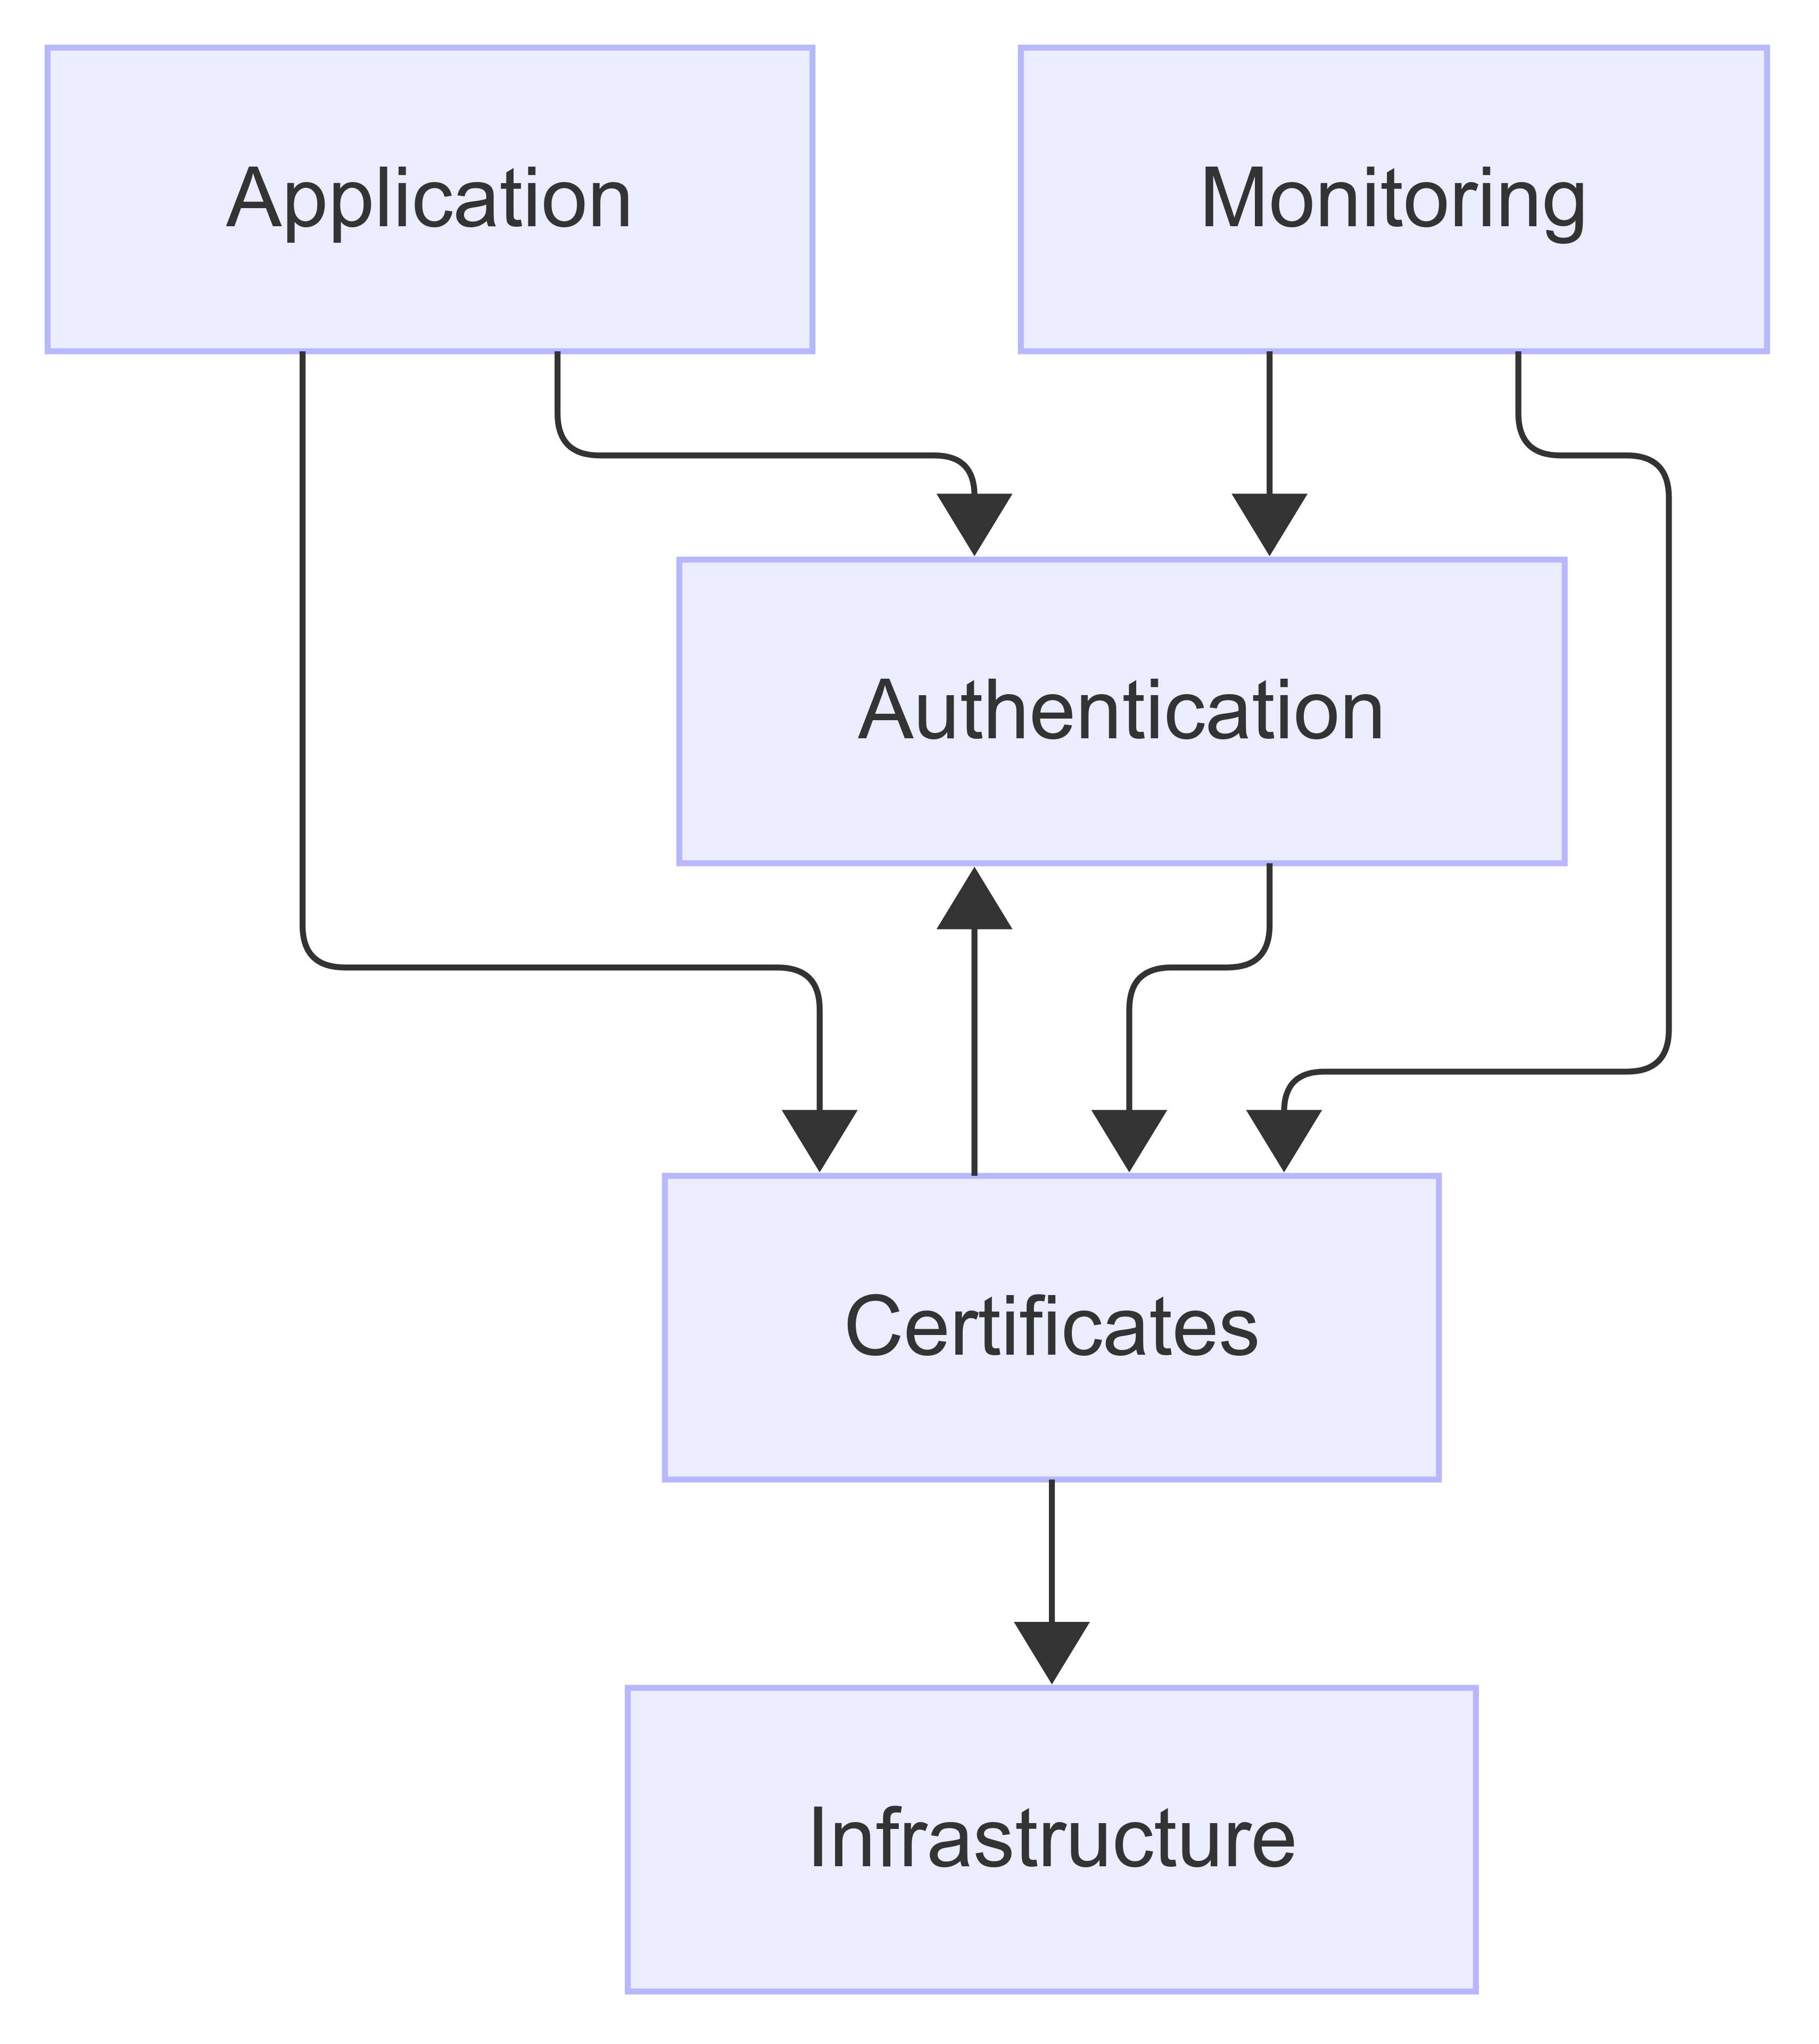
\includegraphics[width=.5\textwidth]{images/pulumi_stacks.png}
    \caption{Pulumi Stacks Relationship. An arrow pointing from a source to a target indicates that the source depends on the target. Given the layered approach, these relationships are transitive. However, arrows targeting certificates are explicitly included due to their significance.}
    \label{fig:pulumi_stacks}
\end{figure}

Our project consists of five Pulumi projects, each with a specific role to play:

\begin{itemize}
    \item \textbf{Application:} Home to CTF platform/cloud-specific functionality.
    \begin{itemize}
        \item \textbf{Homepage:} A user guide for navigating and utilizing the platform.
        \item \textbf{SSHD Alpine bastion:} A secure SSHD server based on Alpine Linux, serving as a bastion host for your cloud environment.
        \item \textbf{CTFd:} A CTF platform for hosting cybersecurity challenges and competitions.
        \item \textbf{Deployer Backend:} The backend service providing core functionality and APIs for the platform.
        \item \textbf{SSLH protocol multiplexer:} A protocol multiplexer that allows multiple services to share a single port, such as SSH and HTTPS.
        \item \textbf{NGINX Proxies:} Proxies to upgrade connection and/or move SSL termination to pod.
        \item \textbf{Unleash:} An open-source solution for feature flagging.
    \end{itemize}
    \item \textbf{Authentication:} Manages SSO capabilities provided by Keycloak.
    \begin{itemize}
        \item \textbf{Keycloak:} An open-source identity and access management solution for Single Sign-On (SSO), enabling secure authentication and authorization.
    \end{itemize}
    \item \textbf{Certificates:} Handles certificate CA and issuers.
    \begin{itemize}
        \item \textbf{Step Certificates:} A Certificate Authority (CA) toolkit for managing and issuing certificates within your environment.
        \item \textbf{Step Autocert:} Automates the issuance and renewal of TLS certificates to ensure your services remain secure.
        \item \textbf{Step Issuer:} An issuer that integrates with Cert-Manager to manage certificate lifecycles.
        \item \textbf{Cert-Manager:} A Kubernetes add-on to automate the management and issuance of TLS certificates from various issuing sources.
    \end{itemize}
    \item \textbf{Infrastructure:} Takes care of basic cluster configuration.
    \begin{itemize}
        \item \textbf{Rancher Local Path Storage Provisioner:} Manages dynamic storage provisioning for Kubernetes using NFS, enabling shared storage across nodes.
        \item \textbf{Nginx Ingress Controller:} Manages external access to services in a Kubernetes cluster through HTTP and HTTPS.
        \item \textbf{KubeVirt:} Extends Kubernetes by adding support for running virtual machine workloads alongside container workloads.
    \end{itemize}
    \item \textbf{Monitoring:} Ensures cluster observability and log collection.
    \begin{itemize}
        \item \textbf{Prometheus:} A monitoring system and time-series database for capturing metrics and alerts.
        \item \textbf{Prometheus-Operator:} Simplifies the setup and management of Prometheus instances within Kubernetes.
        \item \textbf{Grafana:} An open-source platform for monitoring and observability, providing dashboards and visualizations for your metrics.
        \item \textbf{Loki:} A log aggregation system designed for efficiency and ease of use, seamlessly integrating with Prometheus.
        \item \textbf{Promtail:} An agent that ships the contents of local logs to a Loki instance.
        \item \textbf{Node-exporter:} Exports hardware and OS metrics exposed by Linux kernels for monitoring.
    \end{itemize}
\end{itemize}

\subsection{Managing Secrets in Pulumi}
Pulumi includes a built-in mechanism for managing secrets. The user provides a passphrase, which is combined with the encryption salt stored in each stack to encrypt secrets. However, these stacks can also include configuration values in plain text. Secrets can be added using the following command:

\begin{minted}{bash}
    pulumi config set --stack <stack> --secret <key> <value>
\end{minted}

And configuration values can be added using the following command:

\begin{minted}{bash}
    pulumi config set --stack <stack> <key> <value>
\end{minted}

This mechanism functions similarly to a password vault, where all secrets are safeguarded by a single master passphrase. As such, it is crucial to ensure that this passphrase is never compromised. While passwords within the stack can be rotated, the passphrase represents a single point of failure.

In case the passphrase have been compromised, it can be updated using the command:

\begin{minted}{bash}
    pulumi stack change-secrets-provider passphrase --stack <stack>
\end{minted}

Only passwords that must be explicitly known, such as Keycloak login credentials, are stored within the stacks. Passwords that only need to be used by the system are generated during deployment. For example, knowing the database password provides no benefit since it is solely used by the application. Similarly, client credentials for OAuth2 clients are designed to remain confidential. By ensuring that these passwords are not accessible, the risk of them being leaked is eliminated, at least to some extent -- any application can be compromised from within.

Generating secrets during deployment streamlines password rotation. Updating the Infrastructure stack triggers the creation of new credentials, and updating referencing stacks applies these changes. However, Kubernetes does not always restart services automatically, so a rollout restart may be necessary to ensure the updates take effect.

A key word to remember here is \textit{Stack Reference}. When working with micro-stacks, it may be necessary to share information between stacks -- this is trivially given when working with a monolithic approach, as everything is in the same stack. Stack references enable you to access outputs of one stack from another stack. These outputs could include the name of a randomly generated secret, secret values, or any other user-defined stack output.

\chapter{Discussion}

\chapter{Conclusion}

\cleardoublepage
\phantomsection
\addcontentsline{toc}{chapter}{References}
\printbibliography
\end{document}


\chapter{Kubernetes}

\section{Helm Chart}

\section{Horizontal Scaling}

\section{Vertical Scaling}

\section{Health Check}

\section{Probes}

\subsection{Liveness}

\subsection{Readiness}

\subsection{Statup}

\chapter{Development Environment}

\section{Automated Tasks}

\section{Domains}

\chapter{Infrastructure as Code}

\section{Pulumi}

\section{Alternatives}

\section{Developing a Provider}

\chapter{UCloud}

\section{Limited Network Access}

\section{Starting a Virtual Machine}

\section{Domain Name}

\chapter{Monitoring}
Monitoring is an essential aspect of managing a Kubernetes cluster. It provides a comprehensive overview of the health and performance of our services, enabling us to detect and address anomalies before they escalate into critical issues. Effective monitoring allows us to be proactive, ensuring the stability and reliability of our production environment. Rather than reacting to problems like firefighters, we aim to prevent issues from occurring in the first place.

In this chapter, we will explore the various technologies and tools used to achieve effective monitoring. Whether it involves sampling health metrics or gathering logs, the information should be accessible from a single entry point. Dashboards play a crucial role in this process, enhancing and contextualizing the data to make it meaningful and actionable. By leveraging these tools, we can maintain a robust and resilient Kubernetes cluster.

\section{A Single Entry Point}
Monitoring should be straightforward; otherwise, people will not use it! While the initial setup requires some effort, once it is running, all data should be readily available. Therefore, we want all our monitoring to be accessible from a single entry point, so that responsible personnel will not have to aggregate multiple sources to make a rational conclusion about the Kubernetes cluster's health.

To achieve this single entry point, we will use the AIOps tool Grafana. Originally created as a fork of Kibana in 2014, Grafana has since specialized in integrating compatibility with multiple data sources, whereas Kibana is primarily compatible with Elasticsearch. Grafana's ability to support multiple data sources makes it a flexible and future-proof solution.

As a starting point, we will configure Prometheus, Loki, and possibly some databases as data sources. Prometheus is a time series database that collects various metrics. Loki is a system that collects and organizes log data for easy searching and viewing. The purpose of registering databases will primarily be for querying purposes, similar to tools like Adminer.

However, data sources alone will not suffice. As the name suggests, they are simply sources. The data needs to come from somewhere. Prometheus depends on Service Monitors or Pod Monitors to gather metrics, and Loki similarly relies on a log gatherer to collect and organize log data. Without these components, the data sources would remain empty and ineffective. Let us further explore the remaining tool stack in section \ref{sec:monitoring_stack}.

\section{The Technology Stack}\label{sec:monitoring_stack}
In this section, we will explore the use of tools developed by the Grafana and Prometheus community to monitor our Kubernetes cluster. To ensure comprehensive metric sampling, we will utilize various components to collect logs and scrape endpoints provided by the Kubernetes cluster. Below is an overview of the tools we will be using:

\begin{enumerate}
    \item \textbf{Promtail}: Promtail is an agent that ships the contents of local logs to a Loki instance. It is responsible for discovering targets, attaching labels, and pushing logs to the Loki instance.
    \item \textbf{Loki}: Loki is a horizontally-scalable, highly-available log aggregation system inspired by Prometheus. It is designed to be cost-effective and easy to operate, focusing on indexing metadata rather than the full text of the logs.
    \item \textbf{Prometheus}: Prometheus is an open-source systems monitoring and alerting toolkit. It collects and stores metrics as time series data, recording information with a timestamp.
    \item \textbf{Grafana}: Grafana is an open-source platform for monitoring and observability. It provides tools to query, visualize, alert on, and understand your metrics no matter where they are stored.
    \item \textbf{Component scraping the kubelet and kubelet-hosted cAdvisor}: This component scrapes metrics from the kubelet and cAdvisor, which provide information about the resource usage and performance of containers.
    \item \textbf{Component scraping the kube controller manager}: This component collects metrics from the Kubernetes controller manager, which manages the state of the cluster.
    \item \textbf{Component scraping CoreDNS or kubeDNS}: This component gathers metrics from CoreDNS or kubeDNS, which are responsible for DNS-based service discovery in the cluster.
    \item \textbf{Component scraping etcd}: This component scrapes metrics from etcd, the key-value store used as Kubernetes' backing store for all cluster data.
    \item \textbf{Component scraping the kube scheduler}: This component collects metrics from the Kubernetes scheduler, which assigns pods to nodes.
    \item \textbf{Component scraping the kube proxy}: This component gathers metrics from the kube proxy, which maintains network rules on nodes.
    \item \textbf{Component scraping kube state metrics}: This component collects metrics about the state of the Kubernetes objects, such as deployments, nodes, and pods.
    \item \textbf{Deploy node exporter as a daemonset to all nodes}: Node exporter runs on each node to expose hardware and OS metrics.
    \item \textbf{Prometheus Operator}: The Prometheus Operator simplifies the deployment and management of Prometheus and related monitoring components.
\end{enumerate}

The scraping components consist of a service, an associated service monitor, and in some cases, an Endpoints resource. These components are crucial for gathering metrics from various parts of the Kubernetes cluster.

To ensure comprehensive monitoring, we employ both active (intrusive) and passive (non-intrusive) monitoring techniques. Active monitoring involves modifying code to record specific metrics and send information to a logging system, which provides detailed, application-specific insights but adds some overhead. Passive monitoring, on the other hand, collects metrics from the system running the container or VM without modifying the application, offering a broader but more generic view. An example of intrusive monitoring is the metrics endpoint on Loki or Prometheus, while passive monitoring is exemplified by the CAdvisor integrated into the Kubelet, which monitors container resource usage without the containers being aware. By combining both methods, we achieve a balanced and effective monitoring strategy.

As mentioned in the introduction, we have decided to rely primarily on Helm charts when possible. Grafana and Prometheus provide and maintain excellent Helm charts that include features such as horizontal scaling, network policies, and cluster roles. These resources would be complex to create ourselves, so it is beneficial to leverage these pre-built charts.

However, Helm charts are designed to bundle resources, which raises the question of what should be bundled together. For instance, if Grafana is included in multiple Helm charts, which chart should be responsible for deploying it? In this project, we have decided that Helm charts should be as minimal as possible. If it is straightforward to create the integrations ourselves, that is our preferred approach. Helm charts created for specific services, rather than large bundles, are usually easier to configure and comprehend. Moreover, Helm charts targeting deeper integrations align better with our goal of low coupling and high cohesion. Being less dependent on complex charts makes it easier to add or remove services later, allowing us to stay agile and less committed to existing developments.

We utilized several Helm charts to streamline the deployment and management of our monitoring tools. From the Grafana Helm chart repository (\url{https://grafana.github.io/helm-charts}), we used the charts for Grafana, Loki, and Promtail. Additionally, from the Prometheus Community Helm chart repository (\url{https://prometheus-community.github.io/helm-charts}), we employed the kube-prometheus-stack chart.

While considering log shipping solutions, we evaluated both Promtail and Fluent Bit. Promtail is known for its seamless integration with Loki, making it an ideal choice for Kubernetes environments. On the other hand, Fluent Bit offers high performance and flexibility, capable of forwarding logs to multiple destinations. Ultimately, we chose Promtail for its simplicity and compatibility within the Loki ecosystem, which aligns with our goal of maintaining a cohesive and efficient monitoring setup.

\section{Sidecar Container}
In Kubernetes, sidecar containers are a design pattern where an additional container runs alongside the main application container within the same pod. This pattern extends the functionality of the main application without modifying its code. A common use case for sidecar containers is dynamically loading dashboards into Grafana. This approach is particularly advantageous because it avoids unnecessary rolling updates of Grafana, making it super easy to configure new dashboard resources. For example, if using an external Helm chart with their own custom dashboards for Grafana, made for their service, then the dashboards are easily deployed, as there is no need to change the configuration of the currently running Grafana instance. To achieve this, \texttt{ConfigMaps} containing the dashboards must be labeled appropriately, such as with the label \texttt{grafana\_dashboard}. These \texttt{ConfigMaps} should include key-value pairs where the key is the filename and the value is the JSON content of the dashboard.

The sidecar container used for this purpose is typically based on a general-purpose image like \texttt{kiwigrid/k8s-sidecar}. This container continuously scans for \texttt{ConfigMaps} with the specified label and loads them into Grafana using Grafana's public API. The sidecar container is configured with environment variables that specify how to interact with Grafana, including the Grafana URL and an API key for authentication. The API key is usually stored in a Kubernetes Secret and mounted into the sidecar container.

The sidecar container works by continuously scanning the Kubernetes API for \texttt{ConfigMaps} labeled with \texttt{grafana\_dashboard}. When it detects a \texttt{ConfigMap} with this label, it reads the JSON content and stores it in a specified folder within the pod. The sidecar then uses Grafana's public API to import the dashboards, ensuring that any new or updated dashboards are automatically loaded into Grafana without manual intervention. This approach allows for dynamic management of Grafana dashboards, making it easier to update and maintain them as part of a Kubernetes deployment.

Similar features have been prepared for automatically adding scraping targets to Prometheus. These are known as Service Monitors or Pod Monitors, which will be described in the following two sections.

\section{Custom Resource Definition}
In Kubernetes, when the default resources do not meet specific requirements, it is possible to define custom resources to extend the functionality of the cluster. This capability is leveraged by the Prometheus community to introduce a set of Custom Resource Definitions (CRDs) that facilitate advanced monitoring configurations. These CRDs enable the seamless integration and management of Prometheus and related components within a Kubernetes environment. Although not all CRDs are utilized in every deployment, they are included due to their lightweight nature and the complexity involved in selectively disabling them. The Helm chart containing these CRDs is part of the kube-prometheus-stack.

The primary CRDs introduced by the Prometheus community include:

\begin{enumerate}
    \item \textbf{Prometheus}: Defines a Prometheus instance, allowing configuration of replicas, persistent storage, and alerting mechanisms.
    \item \textbf{Alertmanager}: Manages \texttt{Alertmanager} instances, which handle alerts sent by Prometheus and support high availability configurations.
    \item \textbf{ThanosRuler}: Sets up Thanos Ruler instances for processing recording and alerting rules across multiple Prometheus instances.
    \item \textbf{ServiceMonitor}: Specifies how a set of services should be monitored, including endpoints and scraping intervals.
    \item \textbf{PodMonitor}: Similar to \texttt{ServiceMonitor}, but specifically targets pods for monitoring.
    \item \textbf{Probe}: Defines blackbox probing configurations to monitor endpoints from an external perspective.
    \item \textbf{PrometheusRule}: Manages Prometheus recording and alerting rules.
    \item \textbf{AlertmanagerConfig}: Configures \texttt{Alertmanager} settings, such as routing and notification templates.
    \item \textbf{PrometheusAgent}: Sets up a lightweight Prometheus Agent instance for scraping and forwarding metrics.
    \item \textbf{ScrapeConfig}: Provides additional scraping configurations for Prometheus instances.
\end{enumerate}

The Prometheus Operator periodically scans for \texttt{ServiceMonitors}, which define how services should be monitored. Upon discovery, the operator updates Prometheus with the new scraping targets. This allows services exposing metrics in a text-based exposition format to be dynamically added to Prometheus without modifying its configuration or triggering a rolling update. This approach enhances flexibility and reduces operational overhead in maintaining the monitoring setup.

These CRDs facilitate the Kubernetes-native deployment and management of Prometheus and its ecosystem, streamlining the setup and maintenance of an effective monitoring stack.

Deploying the kube-prometheus-stack with Pulumi can sometimes result in failures when resources using a CRD type are detected before the CRD is created. Pulumi may mark these resources as failed after several attempts, an issue that does not occur with Helm. To mitigate this, we take advantage of the Helm chart's design, which allows individual components to be toggled. The CRDs are deactivated as part of the monitoring project but created as part of the fundamental configuration of the Kubernetes cluster.

\section{Service Monitor}
This section will delve into the definition and use of \texttt{ServiceMonitor}, while also comparing it with \texttt{PodMonitor}.

A \texttt{ServiceMonitor} is a CRD that specifies how groups of services should be monitored. It allows Prometheus to scrape metrics from services by defining endpoints and selectors. Here is an example of how to define a \texttt{ServiceMonitor} using TypeScript:

\begin{minted}{typescript}
new k8s.apiextensions.CustomResource("<resource>", {
    apiVersion: "monitoring.coreos.com/v1",
    kind: "ServiceMonitor",
    metadata: {
        namespace: "<namespace>",
        labels: {
            release: "<releaseName>"
        }
    },
    spec: {
        endpoints: [{
            interval: "30s",
            port: "<DNSLabel>"
        }],
        selector: {
            matchLabels: appLabels
        }
    }
})
\end{minted}

In this example, the \texttt{ServiceMonitor} is configured to scrape metrics every 30 seconds from a specified port. The \texttt{selector} field uses labels to identify the services to monitor.

When defining Service Monitors, it is crucial to consider the release label. The Prometheus Operator will only discover Service Monitors or Pod Monitors that are within its release. Additionally, by default, the Prometheus Operator is configured to discover monitors across all namespaces. However, the Prometheus instance itself will, by default, only add scraping targets for monitors that reside within its own namespace.

When defining endpoints in a \texttt{ServiceMonitor}, you can specify either \texttt{port} or \texttt{targetPort}. The \texttt{port} must be a DNS label string referring to a named port defined in a service, while \texttt{targetPort} can be an integer or string representing the target port of the \texttt{Pod} object\footnote{The port must be specified with the container's port property.} behind the service.

While \texttt{ServiceMonitor} is used to monitor services, \texttt{PodMonitor} is designed to monitor pods. Here are the key differences:

\begin{itemize}
    \item \textbf{ServiceMonitor}: Ideal for monitoring a group of pods behind a service. It simplifies the configuration by using service labels and is useful when you want to get a collective measure of the pods running behind a service.
    \item \textbf{PodMonitor}: Suitable for monitoring individual pods directly. It is useful when you need to scrape metrics from specific pods without defining a service. For example, monitoring SQL exporters where you want to consistently scrape each pod's \texttt{/metrics} endpoint without being challenged by load balancing.
\end{itemize}

In summary, use \texttt{ServiceMonitor} when you have services managing multiple pods and need aggregated metrics. Use \texttt{PodMonitor} when you need detailed metrics from individual pods, especially when services are not defined or needed. Everything mentioned in this section has been tested through an experiment.

\chapter{Identity \& Access Management}
\section{Protocols}
\todo{Study this}

\section{Realm \& Client}
When deploying Keycloak, we rely on a Helm chart maintained by Bitnami \parencite{bitnami_keycloak}. Keycloak's documentation can be challenging to navigate, making it difficult to compare the Helm chart with the official documentation to determine how to fill in the Helm \texttt{values.yaml} file. However, after some effort, we managed to configure it. This configuration is part of the monitoring Pulumi project. More interesting is how to configure Keycloak itself to ensure reliable integrations with other services.

\newpage

\section{Integrations}
The significance of Keycloak lies in its practical application. In the following sections, we will explore how Keycloak plays a crucial role in managing authentication for our services. Some open-source software, such as Grafana, allows for seamless integration with Keycloak, making the process straightforward. In contrast, other software solutions, like CTFd, require more effort to integrate. The specifics of these integrations will be detailed in the associated sections.

\subsection{CTFd}
CTFd is arguably our most important exposed service from a practical user perspective. As a web-based platform designed to host CTF competitions, it requires an efficient way to manage users. Ideally, we would leverage external identity providers to avoid the hassle of user creation, relying instead on higher-level institutions or organizations to provide these identities.

However, there is a significant challenge: CTFd does not support any form of SSO unless it is either an enterprise or hosted version \parencite{ctfd_sso}. This limitation forces us to make a choice. Given that CTFd is open-source, we can either 1) modify the source code to implement SSO our way, or 2) create a custom plugin to handle authentication. Modifying the source code would necessitate freezing the version, as future updates could disrupt our changes. Therefore, creating a plugin is the more rational approach.

Fortunately, creating plugins for CTFd is relatively straightforward and well-documented \parencite{ctfd_plugins}. However, there is a notable issue with how the Docker image is developed. Plugin requirements are installed at build time rather than at the entrypoint, which complicates the process. This means we cannot simply mount the plugin to the specified folder without building the Docker file from scratch, as the necessary pip packages are not installed. The solution was to update the entrypoint -- a simple but inconvenient fix\todo{revise}.

The most important detail about the Keycloak plugin developed for CTFd is that it can be configured using the \texttt{config.json} file, and that endpoints can be overwritten as follows:

\begin{minted}{py3}
app.view_functions['auth.login'] = lambda: redirect(url_for('keycloak'))
app.view_functions['auth.logout'] = lambda: redirect(url_for('keycloak_logout'))
app.view_functions['auth.register'] = lambda: ('', 204)
app.view_functions['auth.reset_password'] = lambda: ('', 204)
app.view_functions['auth.confirm'] = lambda: ('', 204)
\end{minted}

When the user clicks the login button, they are redirected to our custom login page instead of the usual login page. The same applies to the logout button. Additionally, endpoints can be disabled in this manner, resulting in a 204 status code (indicating that the request has been successfully processed, but no content is returned). The code block above demonstrates that if the register button is made public during setup, it will not function as it redirects to nowhere. The same logic applies to the reset password and confirm (login callback) endpoints.

The implementation has been done using \texttt{python-keycloak} \parencite{python_keycloak}, a tool specialized for handling authentication with Keycloak, utilizing the \textit{authorization code} grant type. While a more general approach could have involved using a generic OIDC plugin, \texttt{python-keycloak} was chosen for its ease of use and effectiveness in solving our specific problem.

The login flow utilizes the Authorization Code Grant (see Section \ref{sec:auth_code}) and operates as follows:

\begin{enumerate}
    \item A user logs into CTFd using their SSO credentials.
    \item If the user does not exist in CTFd's database, they are created; otherwise, the existing user is fetched.
    \item Roles and other profile settings are synchronized to match the configurations of the SSO user.
    \item The user is then logged into CTFd with their SSO credentials.
\end{enumerate}

If necessary, administrators can disable or ban users from CTFd. It is important to note that even if a user is deleted from CTFd's database, they will be recreated upon logging in again. Conversely, if a user is deleted in Keycloak, they will still exist in CTFd's database but will be unable to log in, as authentication is handled by Keycloak. Therefore, to properly delete a user, they must be removed from both databases, or at least from CTFd's database with their roles revoked to prevent authorization upon authentication.

In SQLAlchemy, \texttt{polymorphic\_on} and \texttt{polymorphic\_identity} are used to handle inheritance in database models. The \texttt{polymorphic\_on} attribute specifies the column used to determine the type of the object, while \texttt{polymorphic\_identity} sets the identity for each subclass. This allows SQLAlchemy to distinguish between different types of objects stored in the same table.

\begin{minted}{py3}
class Users(db.Model):
    __tablename__ = "users"
    __mapper_args__ = {"polymorphic_identity": "user", "polymorphic_on": type}
    ...

class Admins(Users):
    __tablename__ = "admins"
    __mapper_args__ = {"polymorphic_identity": "admin"}
\end{minted}

The \texttt{Submissions} class has a foreign key \texttt{user\_id} that references the \texttt{users} table. The \texttt{ondelete="CASCADE"} ensures that when a user is deleted, all related submissions are also deleted.

\begin{minted}{py3}
class Submissions(db.Model):
    __tablename__ = "submissions"
    id = db.Column(db.Integer, primary_key=True)
    user_id = db.Column(db.Integer, db.ForeignKey("users.id", ondelete="CASCADE"))
\end{minted}

Handling polymorphic types can be challenging, especially when changing the type of an existing object. For example, if you add an admin and later change its type to user, you might encounter an \texttt{ObjectDeletedError}. This error occurs because changing the polymorphic identity can lead to the deletion of the original object, causing issues with related objects like submissions and comments that are linked via foreign keys with cascade delete.

To handle the issue of changing polymorphic types without losing related objects, you can generate the response first before actually changing the type. This avoids the \texttt{ObjectDeletedError}. This solution was found by reading through the source code for CTFd's public API \cite{CTFdUsersAPI}.

\begin{minted}{py3}
def patch_user(user_id, data):
    user = Users.query.filter_by(id=user_id).first_or_404()
    data["id"] = user_id

    schema = UserSchema(view="admin", instance=user, partial=True)
    response = schema.load(data)
    if response.errors:
        return {"success": False, "errors": response.errors}, 400

    # This generates the response first before actually changing the type
    # This avoids an error during User type changes where we change
    # the polymorphic identity resulting in an ObjectDeletedError
    # https://github.com/CTFd/CTFd/issues/1794
    response = schema.dump(response.data)
    ...
\end{minted}

By understanding and properly handling polymorphic types in SQLAlchemy, you can avoid issues like \texttt{ObjectDeletedError} and ensure that related objects are preserved when changing the type of a user. This involves generating responses before changing types and using methods to manage related objects effectively. This approach ensures that properties and linked objects like submissions and comments are not lost during the type change.\todo{explain API keys}

\subsection{Grafana}\label{sec:grafana_auth}
Integrating Grafana with Keycloak addresses the critical challenges of secure and efficient user authentication and authorization by leveraging standardized protocols. This section details the configuration process, focusing on protocol integration, PKCE, refresh tokens, role mapping, and the underlying protocols \parencite{GrafanaKeycloak}.

\begin{minted}{javascript}
{
    "auth.generic_oauth": {
        enabled: true,
        use_pkce: true,
        allow_sign_up: true,
        use_refresh_token: true,
        role_attribute_strict: true,
        client_secret: GRAFANA_CLIENT_SECRET,
        scopes: "openid",
        client_id: "grafana",
        name: "Keycloak-OAuth",
        name_attribute_path: "name",
        email_attribute_path: "email",
        id_token_attribute_name: "access_token",
        login_attribute_path: "preferred_username",
        token_url: `${keycloakIntern}/realms/ctf/protocol/openid-connect/token`,
        auth_url: `${keycloakExtern}/realms/ctf/protocol/openid-connect/auth`,
        api_url: `${keycloakExtern}/realms/ctf/protocol/openid-connect/userinfo`,
        signout_redirect_url: `${keycloakExtern}/realms/ctf/protocol/openid-connect/logout`,
        role_attribute_path: "contains(resource_access.grafana.roles, 'admin') && 'Admin' || contains(resource_access.grafana.roles, 'editor') && 'Editor' || ''"
    }
}
\end{minted}

Grafana integrates with Keycloak using OAuth2 and OIDC. Key endpoints include the authorization endpoint, token endpoint, user info endpoint, and logout endpoint. By setting \texttt{id\_token\_attribute\_name} to \texttt{access\_token}, Grafana uses the access token for authorization, avoiding the need for additional client mappers required by the ID token used by default; otherwise, Grafana will not be able to find the client roles. This approach simplifies the configuration by utilizing the readily available information already in the access token.

Grafana uses the \texttt{sub} claim as the unique identifier for the user. This can be changed to the email by setting \texttt{oauth\_allow\_insecure\_email\_lookup} to \texttt{true}. This option is typically used when authenticating with different identity providers. However, it is noteworthy that user synchronization issues may arise if the basic claim scope is missing \parencite{grafana_authentication}.

PKCE enhances the security of the OAuth2 authorization code flow, particularly for public clients. It mitigates authorization code interception attacks by introducing a code verifier and code challenge. The client generates a code verifier and sends a hashed code challenge to the authorization server. Upon exchanging the authorization code for an access token, the client presents the original code verifier. This ensures that intercepted authorization codes cannot be used without the code verifier, significantly enhancing security.

Refresh tokens maintain user sessions without frequent re-authentication. Upon initial login, both an access token and a refresh token are issued. The access token has a short lifespan, while the refresh token is long-lived. When the access token expires, the client uses the refresh token to obtain a new access token, ensuring continuous access and improving user experience while maintaining security.

Role mapping in Grafana is achieved using JMESPath, a query language for JSON. The \texttt{role\_attribute\_path} configuration extracts and maps roles from the Keycloak token to Grafana roles. This path dynamically maps Keycloak roles to Grafana roles, ensuring accurate user permissions.

Integrating Grafana with Keycloak for authentication provides a secure and efficient solution for managing user access in modern web applications. By leveraging OAuth2 and OIDC protocols, utilizing PKCE, implementing refresh tokens, and employing dynamic role mapping, this integration enhances security and user experience, ensuring that only authorized users can access sensitive data visualized in Grafana.

\subsection{Step Certificates}

\subsection{APIs}

\chapter{Certificate Management}

It’s both. The CRD (Custom Resource Definition) StepIssuer defines how cert-manager interacts with the step issuer, and using cert-manager.io/v1 as the API version ensures that cert-manager processes the certificate request.

The StepIssuer CRD is what allows cert-manager to understand and utilize Step Issuer-specific configurations. The apiVersion specifies that this CRD is part of cert-manager’s ecosystem, linking the certificate management workflow to the Step Issuer capabilities.

So, it’s the combination of the StepIssuer CRD defining the step-issuer's specifics and the API version that ties it into cert-manager’s functionality.

\section{Zero Trust}

\section{Certificate Authority}

\section{ACME for TLS}

\section{SSH Certificates}

\section{Smallstep}

\subsection{Smallstep SSH}

\subsection{Step Certificates}

\subsection{Autocert}

\subsection{Issuer}

\subsection{Bootstrap}

\begin{minted}{bash}
fingerprint=$(
    curl -k https://myhost/roots.pem | 
    openssl x509 -noout -sha256 -fingerprint | 
    sed 's/://g' | 
    tr 'A-F' 'a-f' | 
    awk -F= '{print $2}'
)

step ca bootstrap --ca-url https://myhost \
    --fingerprint $fingerprint \
    --force \
    --install
\end{minted}


% https://github.com/smallstep/cli/blob/3d38cfeadb8f90e8b916a7b7e9c1d4fe9e80a43f/command/oauth/cmd.go#L331

% step will expect to be able to perform a TLS handshake with the proxy, and use the CA's root certificate to complete the trust chain. So, for inbound TLS connections, the proxy should use a server certificate issued by step-ca. See below for an example.

% Layer 4 (Transport Layer): This deals with transportation of data between systems. It doesn’t concern itself with what the data is, but with the movement of the data packets. In a layer 4 proxy, this means forwarding traffic based purely on TCP/UDP protocols without looking at the actual content. This is often referred to as "TLS passthrough" because the proxy doesn’t terminate the SSL/TLS connection—it just passes it through to the backend server.

% Layer 7 (Application Layer): This goes a step further, inspecting and potentially modifying the data itself because it operates at the application level. A layer 7 proxy can make decisions based on HTTP headers, cookies, and other data in the web traffic, allowing for more sophisticated routing and filtering. The proxy terminates the SSL/TLS connection, decrypts the data, and then possibly re-encrypts it before sending it to the backend server.

% Layer 1 - Physical: Deals with the physical connection between devices, including cables and switches.

% Layer 2 - Data Link: Manages data transfer between adjacent network nodes, using MAC addresses.

% Layer 3 - Network: Handles routing of data packets using IP addresses.

% Layer 4 - Transport: Ensures reliable data transfer with error correction and flow control (e.g., TCP/UDP).

% Layer 5 - Session: Manages sessions or connections between applications.

% Layer 6 - Presentation: Translates data between the application layer and the network, dealing with data encryption and compression.

% Layer 7 - Application: Provides network services directly to end-user applications, such as web browsers and email clients.

% The Root function in the step-ca client code requires no TLS termination because it relies on a direct, secure connection to the CA to ensure the integrity and authenticity of the root certificate. Here’s a detailed explanation:

% Key Points of the Root Function
% Direct HTTPS Request:
% Go

% resp, err := c.httpClient.Get(c.baseURL + "/root/" + fingerprint)
% Kode genereret af kunstig intelligens. Gennemse og brug forsigtigt. Flere oplysninger om ofte stillede spørgsmål.
% This line makes an HTTPS request to the CA to retrieve the root certificate. The httpClient is configured to establish a secure TLS connection directly to the CA.
% Certificate Validation:
% Go

% defer resp.Body.Close()
% // Parse and validate the certificate
% Kode genereret af kunstig intelligens. Gennemse og brug forsigtigt. Flere oplysninger om ofte stillede spørgsmål.
% After receiving the response, the function parses and validates the certificate. This validation process ensures that the certificate matches the expected fingerprint and is trusted.
% Why No TLS Termination is Required
% End-to-End Encryption:
% The Root function expects the entire communication path to be encrypted from the client to the CA. TLS termination at the ingress would break this end-to-end encryption, as the ingress would decrypt and then re-encrypt the traffic. This intermediate step can introduce security risks and prevent the client from validating the CA’s certificate directly.
% Certificate Integrity:
% The client needs to ensure that the root certificate it receives is authentic and has not been tampered with. By maintaining a direct TLS connection, the client can securely retrieve and validate the certificate against the provided fingerprint. Any interruption in this secure channel could compromise the integrity of the certificate.
% Security Policies:
% The step CLI and step-ca are designed with strict security policies that require direct, secure communication with the CA. Allowing TLS termination would violate these policies and potentially expose the communication to man-in-the-middle attacks.
% Summary
% In summary, the Root function requires a direct, uninterrupted TLS connection to ensure the security and integrity of the root certificate retrieval process. SSL passthrough is necessary to maintain this secure connection from the client to the CA, preventing any intermediate decryption and re-encryption that could compromise the security.

% // BootstrapClient is a helper function that using the given bootstrap token
% // return an http.Client configured with a Transport prepared to do TLS
% // connections using the client certificate returned by the certificate
% // authority. By default the server will kick off a routine that will renew the
% // certificate after 2/3rd of the certificate's lifetime has expired.
% //
% // Usage:
% //
% //	// Default example with certificate rotation.
% //	client, err := ca.BootstrapClient(ctx.Background(), token)
% //
% //	// Example canceling automatic certificate rotation.
% //	ctx, cancel := context.WithCancel(context.Background())
% //	defer cancel()
% //	client, err := ca.BootstrapClient(ctx, token)
% //	if err != nil {
% //	  return err
% //	}
% //	resp, err := client.Get("https://internal.smallstep.com")
% func BootstrapClient(ctx context.Context, token string, options ...TLSOption) (*http.Client, error) {
% 	b, err := createBootstrap(token) //nolint:contextcheck // deeply nested context; temporary
% 	if err != nil {
% 		return nil, err
% 	}

% 	// Make sure the tlsConfig has all supported roots on RootCAs.
% 	//
% 	// The roots request is only supported if identity certificates are not
% 	// required. In all cases the current root is also added after applying all
% 	// options too.
% 	if !b.RequireClientAuth {
% 		options = append(options, AddRootsToRootCAs())
% 	}

% 	transport, err := b.Client.Transport(ctx, b.SignResponse, b.PrivateKey, options...)
% 	if err != nil {
% 		return nil, err
% 	}

% 	return &http.Client{
% 		Transport: transport,
% 	}, nil
% }


% The real trust chain verification happens because of the setup performed by the transport layer. Here’s how it works:

% Add Root Certificate:

% go

% Kopiér
% options = append(options, AddRootsToRootCAs())
% This function ensures the root certificate is included in the client's trust store, making it available for the TLS handshake.

% Transport Configuration:

% go

% Kopiér
% transport, err := b.Client.Transport(ctx, b.SignResponse, b.PrivateKey, options...)
% This sets up the transport layer with the necessary certificates and keys. The Transport method configures the client to use these certificates for TLS connections.

% TLSConfig Setup: The Transport function uses the root certificate to create a tls.Config object. This object is part of the Go standard library and handles the TLS handshake.

% Here's a snippet of what happens under the hood in the Transport method:

% go

% Kopiér
% tlsConfig := &tls.Config{
%     Certificates: []tls.Certificate{clientCert},
%     RootCAs:      rootCertPool,
% }
% TLS Handshake: When the client makes a request, the tls.Config object handles the TLS handshake, verifying the server’s certificate against the root certificates in the rootCertPool.

% So, the key part of the process is the creation and configuration of the tls.Config object, which includes the root certificate and client certificate. This configuration allows the TLS handshake to verify the server certificate and complete the trust chain


% Ah, let me clarify that. The BootstrapServer function in step-ca sets up the server's TLS configuration, ensuring it can handle secure inbound TLS connections. This is more about the server's preparation to securely interact with clients.

% When you use the step ca bootstrap command with the step-cli, it interacts with the step-ca server to download the root certificate and configure the client environment. The client-side setup is done by the BootstrapClient function, ensuring the client can make secure connections to the server.

% So, while BootstrapServer prepares the server, the client’s bootstrap process is handled by BootstrapClient. Both sides work together to ensure secure communication, but they handle different parts of the setup.


% Yes, you’ve got it! When the BootstrapClient function returns an http.Client object, it’s the step-cli that receives it. Specifically, the step-cli uses this returned http.Client to make secure HTTP requests to the step-ca server.

% So, the client configured by BootstrapClient allows the step-cli to securely communicate with the CA server, leveraging the configured TLS settings to ensure the trust chain is validated.


% "command": "/bin/bash -c \"echo $name:*:19156:0:99999:7:::\""

% That string of numbers and symbols represents various fields in the shadow file entry. Here's a breakdown:

% $name: Username.

% *: Password field (an asterisk means no password is set).

% 19156: Days since the Unix epoch (1 January 1970) when the password was last changed.

% 0: Minimum number of days before a password change is allowed.

% 99999: Maximum number of days the password is valid.

% 7: Number of days before the password expires that the user is warned.

% :::: These fields are left blank, typically for inactivity period, expiration date, and reserved for future use.

% Each field has a specific purpose in managing user passwords and their expiration policies. It's part of the system's security mechanisms. Quite the intricate dance of digits and colons!


% TODO remembe to discuss that the CTFd OIDC auth does not conflict with API

% CORS, same-site cookie attribute and same-origin policy

% sudo apt-get install libvirt-clients
% virt-host-validate qemu